\documentclass[11pt]{article}
\usepackage{inputenc}
\usepackage{comment}
\usepackage{fontspec}
\usepackage{authblk}
\usepackage{graphicx}
\usepackage{fancyhdr}
\usepackage{amssymb}
\usepackage{amsmath}
\usepackage{gensymb}
\usepackage{float}
\usepackage{enumerate}
\usepackage{tocloft}
\usepackage{abstract}
\usepackage[hidelinks]{hyperref}
\usepackage{appendix}
\usepackage[dvipsnames, svgnames, x11names]{xcolor}
\usepackage{dirtree}
\usepackage{cite}
\usepackage{geometry}
\usepackage{makecell}
\usepackage{multirow}
\usepackage{graphicx}
\usepackage{float}
\usepackage{subfig}
\usepackage[ruled]{algorithm2e}
\usepackage{indentfirst}
\usepackage{unicode-math}
\usepackage{afterpage}
\usepackage{tikz}

\usepackage{setspace}

\setlength{\headheight}{16pt}

\setmainfont[%
ItalicFont=NewCM10-Italic.otf,%
BoldFont=NewCM10-Bold.otf,%
BoldItalicFont=NewCM10-BoldItalic.otf,%
SmallCapsFeatures={Numbers=OldStyle}]{NewCM10-Regular.otf}

\setsansfont[%
ItalicFont=NewCMSans10-Oblique.otf,%
BoldFont=NewCMSans10-Bold.otf,%
BoldItalicFont=NewCMSans10-BoldOblique.otf,%
SmallCapsFeatures={Numbers=OldStyle}]{NewCMSans10-Regular.otf}

\setmonofont[ItalicFont=NewCMMono10-Italic.otf,%
BoldFont=NewCMMono10-Bold.otf,%
BoldItalicFont=NewCMMono10-BoldOblique.otf,%
SmallCapsFeatures={Numbers=OldStyle}]{NewCMMono10-Regular.otf}

\setmathfont{NewCMMath-Regular.otf}

\pagestyle{fancy}

\renewcommand\thesection{\arabic{section}}

\newcommand*{\rmd}{\mathop{}\!\mathrm{d}}
\newcommand*{\sgn}{\mathrm{sgn}}
\renewcommand{\cftsecleader}{\cftdotfill{\cftdotsep}}

\title{\Huge Project Report}

\author{
  \parbox{\textwidth}{
    \vspace{0.5cm}
    \centering \LARGE Team \#12
    \vspace{0.5cm}
  } \\
  \parbox{0.2\textwidth}{
    \centering WANG Zeyu
  }
  \parbox{0.2\textwidth}{
    \centering YANG Xirui
  }
  \parbox{0.2\textwidth}{
    \centering Wu Tianxiao
  }
}

\date{\today}

\setcounter{tocdepth}{2}
\setcounter{secnumdepth}{3}

\begin{document}

\maketitle
\thispagestyle{empty}
\setcounter{page}{0}

\vspace{1cm}

\begin{abstract}
  This report presents our team's solutions of three classification tasks: student placement prediction, feature-based multi-class classification, and fraud detection. We first introduce the problem definition and the dataset as well as give a brief introduction of the methods we use. Then the for each task, following the data analytical process, we design the preparing and analyzing algorithm to handle the problems such as the missing values and feature engineering. We use the techniques like correlation coefficient and $k$ nearest neighbor imputer in exploration and preprocessing, then the logistics regresson, decision tree and multilayer perceptron are implement and apply to the data. In the end, we report the model performance with the discovery based on the results.
  \\\\
  \textbf{Keywords:} Classification, Machine learning.
\end{abstract}

\newpage

\section{Problem Definition}

\subsection{Task 1}

\subsection{Task 2}

\subsection{Task 3}

\section{Data Prepare}

\subsection{Correlation coefficient}

The correlation coefficient measures the relationship between two samples, which can also be used to find the potential relationship between features and labels in classification tasks. Pearson correlation coefficient, Kendall correlation coefficient and Spearman correlation coefficient are three of mostly used methods, which indicate the linear and rank correlation between features and labels.

\subsubsection{Pearson correlation coefficient}

Given two samples ${x}_{i=1}^n, {y}_{i=1}^n$ with size $n$, the Pearson correlation coefficient measures the correlation via

$$
  r (x, y) = \frac{\sum_{i=1}^n (x - \bar{x}) (y - \bar{y})}{\sqrt{\sum_{i=1}^n (x_i - \bar{x})^2} \sqrt{\sum_{i=1}^n (y_i - \bar{y})^2}},
$$

\noindent where $\bar{x} = \frac{1}{n} \sum_{i=1}^n$ is the sample mean of $x$, and analogously for $\bar{y}$.

The values of the Pearson correlation coefficients are within range $[-1, 1]$ and the absolute value indicates the level of correlation. This is a commonly used method to find the potential relationship between the features, but it can only handle the linear relationship, while the nonlinearity, noise and outliers can lead to a incorrect result.

\subsubsection{Kendall \& Spearman correlation coefficient}

The Kendall correlation coefficient and Spearman correlation coefficient are both rank correlation coefficient, which measured the similarity between two rankings, i.e., whether the rank of one sample correspond to the rank of another sample. Based on this idea, these correlation coefficients are more robust to outliers, and effective for monotonic relationships.

Given two samples ${x}_{i=1}^n, {y}_{i=1}^n$ with size $n$ and unique elements, the Kendall correlation coefficient is computed based on the Pearson correlation coefficient between the rank variables as

$$
  r_k (x, y) = \frac{\#(\text{Concordant pairs}) - \#(\text{Discordant pairs})}{\#(\text{All paires})},
$$

where $\#(\cdot)$ calculate the number of the elements in the set, and a pair $(i, j), i < j$ is concordant if $x_i < x_j, y_i < y_j$ or $x_i > x_j, y_i > y_j$, otherwise discordant. This method can also be expanded to the non-unique values.

Given two samples ${x}_{i=1}^n, {y}_{i=1}^n$ with size $n$, the Spearman correlation coefficient is computed based on the Pearson correlation coefficient between the rank variables as

$$
  r_s (x, y) = r(R(x), R(y)),
$$

where $R(x)$ and $R(y)$ are the rank of the samples.

\subsection{$k$ nearest neighbors imputer}

The $k$ nearest neighbors imputer fill in the missing values based on the $k$ nearest neighbors algorithm. With the euclidean distance metric that supports missing values, which compute the distance with existing features, each missing value is imputed using the mean value of nearest neighbors.

This method works with both numerical and categorical data, but can be easily influenced by the distribution of the data especially when the data is sparse in the nearby area.

\subsection{Dimension raising}

In order to better deal with the nonlinearity, we used the dimension raising in preprocessing, which transform the data to a higher dimensional space. Given the scalar data $x_i$ and a given degree $d$, one simple way is to compute the new data as $(x_i, x_i^2, \dots, x_i^d)$, which will make some patterns or relationships more apparent. Another way is to combine the features. Given scalar $x_i$ and $y_i$, the new data is computed as $(x_i, y_i, x_i y_i)$. In this approach, we can manually constructe new features based on the real world infomation, which can better balance the data size and model performance.

The Figure \ref{sample-raising} shows the example for dimension raising. In the origin data (the left figure), the red part is between the two blue part, whcih can make difficulty in classification, especially for linear or weakly nonlinear classifier, while the data after dimension raising can be easily separated.

\begin{figure}[H]
  \centering
  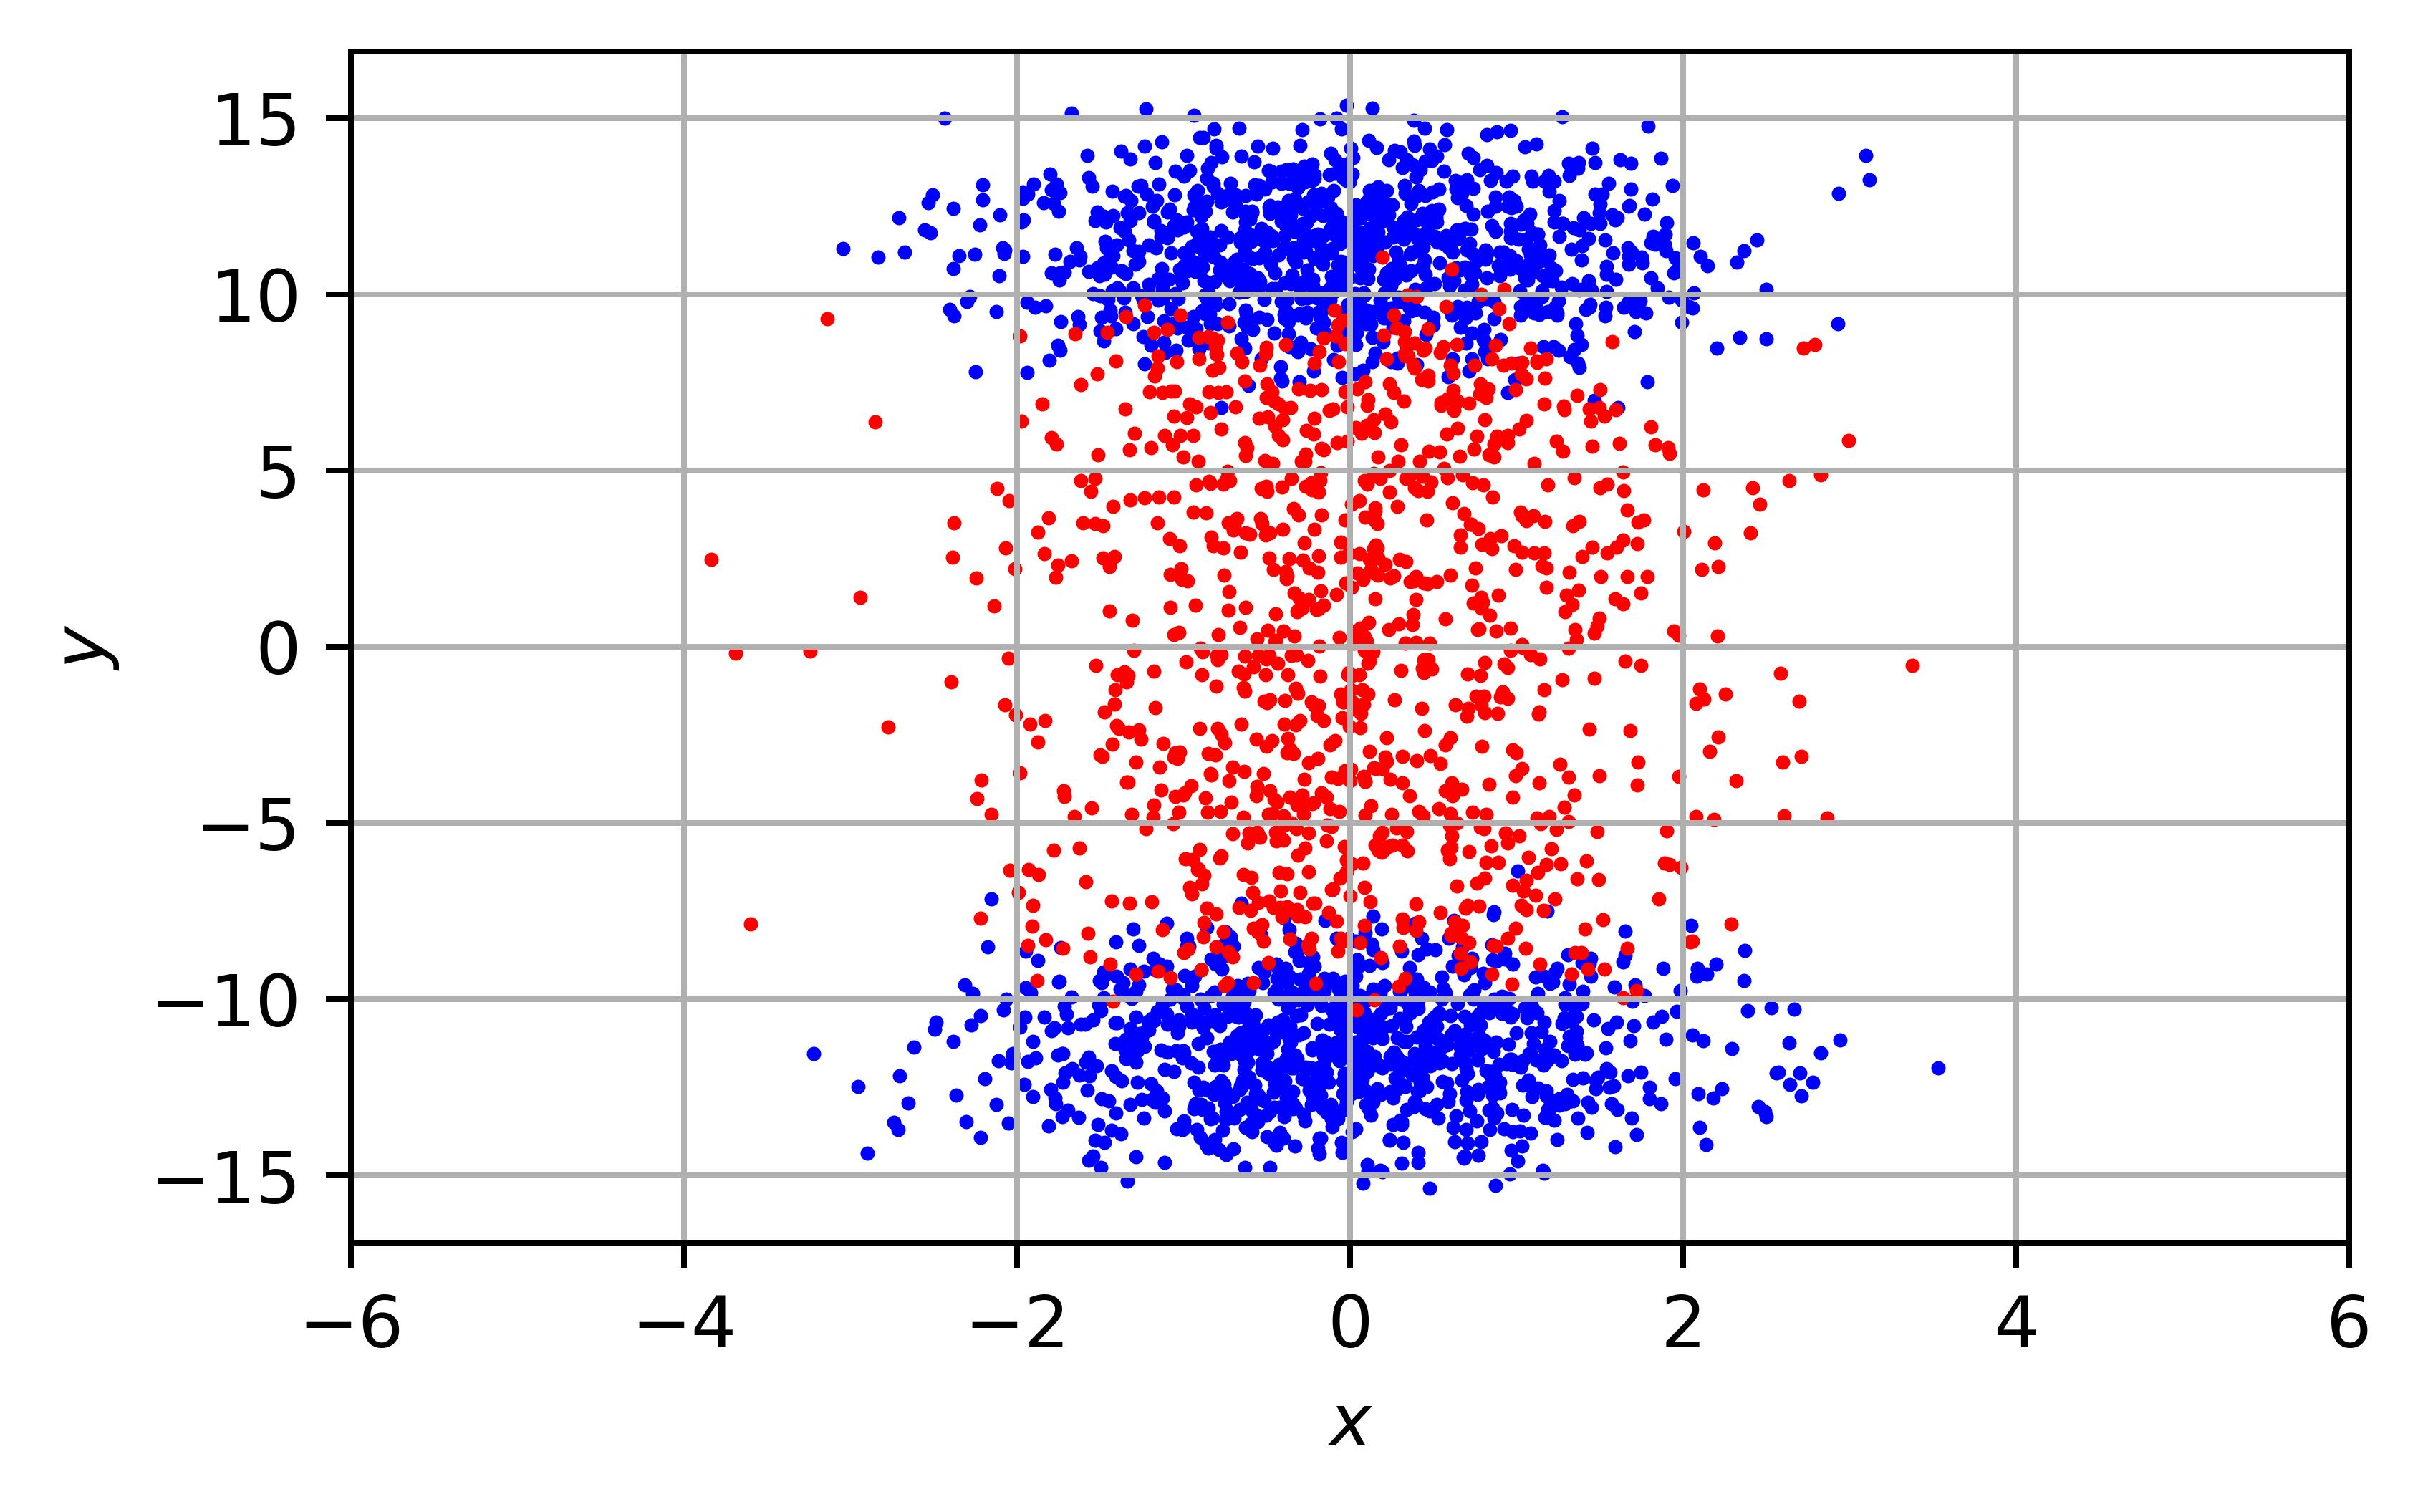
\includegraphics[width=0.4\textwidth]{./figure/Sample-Raising-1.jpg}
  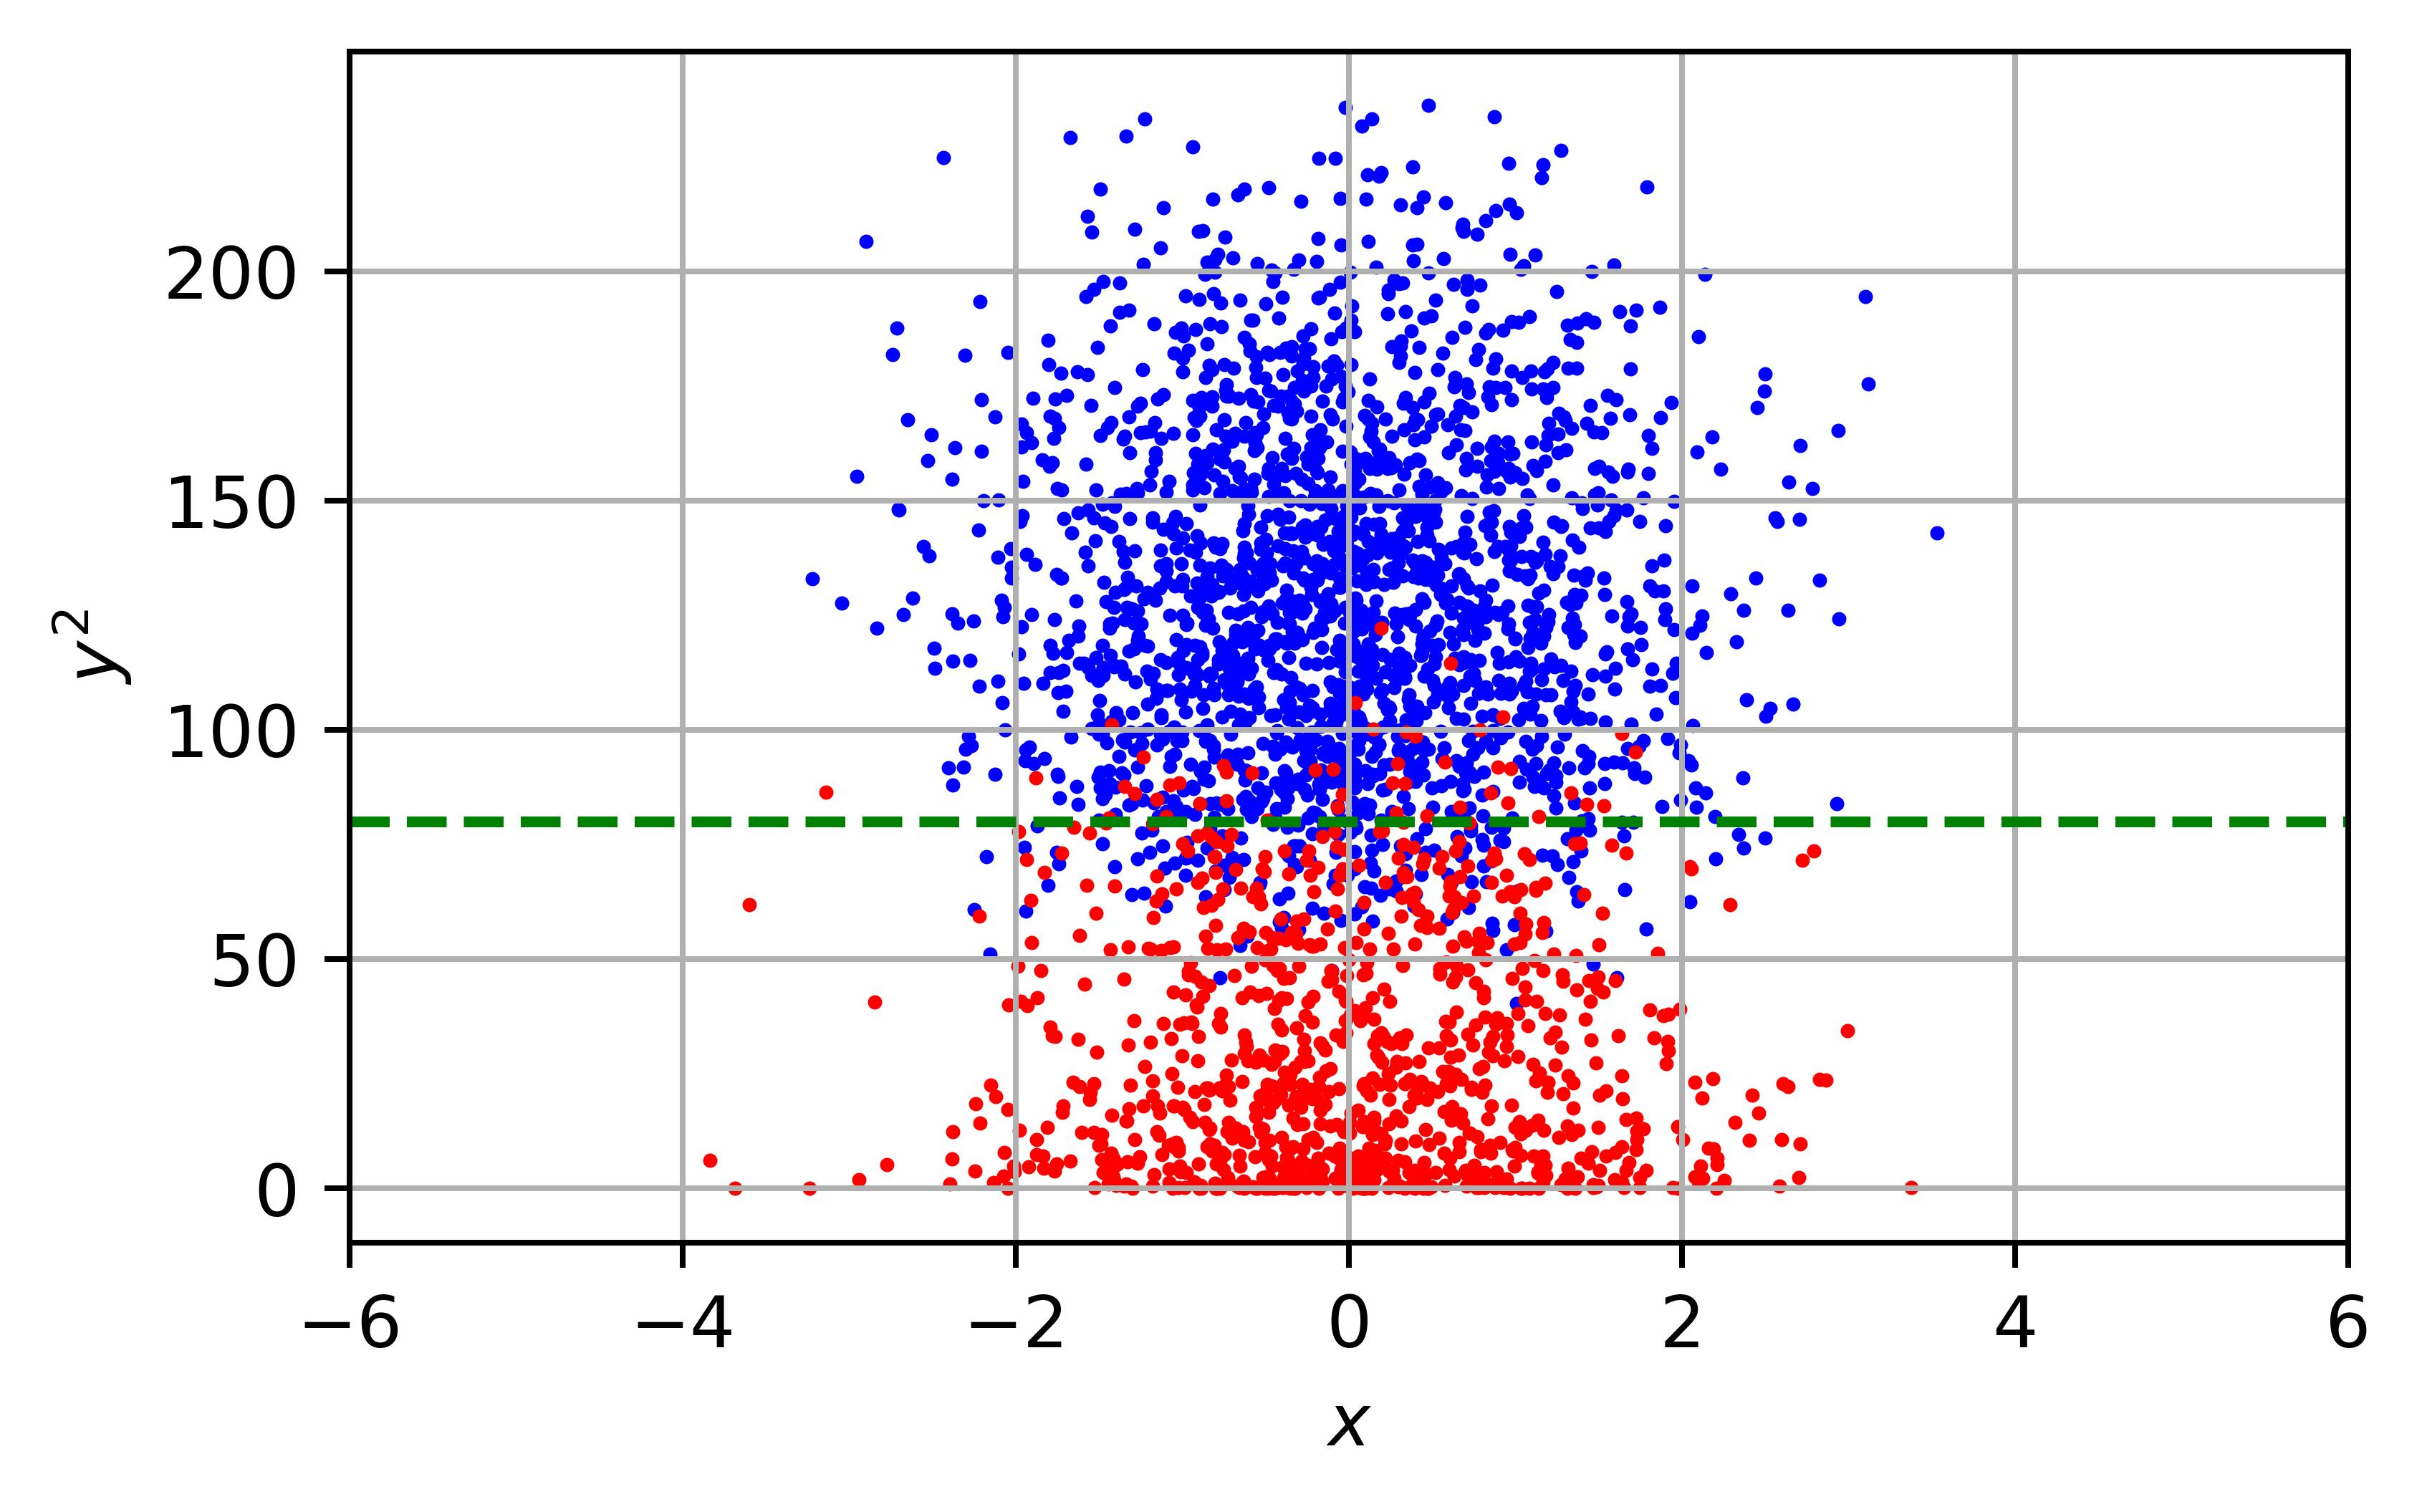
\includegraphics[width=0.4\textwidth]{./figure/Sample-Raising-2.jpg}
  \caption{Example for dimension raising. The left shows that origin data, where the data is not linearly separable, while the right shows the data after dimension raising, where the $y_2$ is easy to be separated by a line.}
  \label{sample-raising}
\end{figure}

\section{Data Analysis}

\subsection{Logistic regression}

The logistic regression is a widely used linear classification model. By linearly combine the input features, the logistic regression gives a probability value ranging between $0$ and $1$ as output. Due to the linearty, this model will be less prone to overfitting, but on the other hand, it can't catch the nonlinearity.

\subsection{Decision tree}

The decision tree is a supervised learning method used for classification. Based on the simple decision rules inferred from the data features, it will create a model that predict the label with piecewise constant approximation.

One of the main property of decision trees is that it don't require data preparation like normalization or standardization of data, further more, it can handle both categorical and numerical data and multi-output problems, which means that some preprocessing, such as one hot encoding, is not necessary.

\subsection{Multilayer perceptron}

The multilayer perceptron (MLP) is a basic kind of neural network which learns a function $f: \mathbb{R}^n \mapsto \mathbb{R}^m$ to approximate the input and output. Differnet from the logistic regression, the MLP includes some hidden layer with the nonlinear active function, which can help handle nonlineariy of the data, as well as the hierarchical feature extraction, i.e., it can capturing increasingly complex patterns level by level.

\section{Implementation}

\subsection{Logistic regression}

\subsection{Decision tree}

\subsection{Multilayer perceptron}

\section{Solution}

\subsection{Task 1}

\subsection{Task 2}

\subsection{Task 3}

\section{Summary}

\newpage

\bibliographystyle{unsrt}
\bibliography{reference.bib}
\addcontentsline{toc}{section}{References}

\newpage

\appendix
\renewcommand\thesection{\Alph{section}}

\section{Author Contributions}

% WANG Zeyu:
% YANG Xirui:
% Wu Tianxiao:

\end{document}